%----------------------------------------------------------------------------------------
% PACKAGES AND OTHER DOCUMENT CONFIGURATIONS
%----------------------------------------------------------------------------------------
\documentclass{article}
\usepackage{fancyhdr} % Required for custom headers
\usepackage{lastpage} % Required to determine the last page for the footer
\usepackage{extramarks} % Required for headers and footers
\usepackage[usenames,dvipsnames]{color} % Required for custom colors
\usepackage{graphicx} % Required to insert images
\usepackage{listings} % Required for insertion of code
\usepackage{courier} % Required for the courier font
\usepackage{lipsum} % Used for inserting dummy 'Lorem ipsum' text into the template
\usepackage[utf8]{inputenc}
\usepackage[ngerman]{babel}
% Margins
\topmargin=-0.45in
\evensidemargin=0in
\oddsidemargin=0in
\textwidth=6.5in
\textheight=9.0in
\headsep=0.25in
\linespread{1.1} % Line spacing
% Set up the header and footer
\pagestyle{fancy}
%\lhead{\hmwkAuthorName} % Top left header
\chead{\hmwkClass\ : \hmwkTitle} % Top center head
\rhead{\firstxmark} % Top right header
\lfoot{\lastxmark} % Bottom left footer
\cfoot{} % Bottom center footer
\rfoot{Page\ \thepage\ of\ \protect\pageref{LastPage}} % Bottom right footer
\renewcommand\headrulewidth{0.4pt} % Size of the header rule
\renewcommand\footrulewidth{0.4pt} % Size of the footer rule
\setlength\parindent{0pt} % Removes all indentation from paragraphs
%----------------------------------------------------------------------------------------
% CODE INCLUSION CONFIGURATION
%----------------------------------------------------------------------------------------
\definecolor{MyDarkGreen}{rgb}{0.0,0.4,0.0} % This is the color used for comments
\lstloadlanguages{Perl} % Load Perl syntax for listings, for a list of other languages supported see: ftp://ftp.tex.ac.uk/tex-archive/macros/latex/contrib/listings/listings.pdf
\lstset{language=Perl, % Use Perl in this example
frame=single, % Single frame around code
basicstyle=\small\ttfamily, % Use small true type font
keywordstyle=[1]\color{Blue}\bf, % Perl functions bold and blue
keywordstyle=[2]\color{Purple}, % Perl function arguments purple
keywordstyle=[3]\color{Blue}\underbar, % Custom functions underlined and blue
identifierstyle=, % Nothing special about identifiers
commentstyle=\usefont{T1}{pcr}{m}{sl}\color{MyDarkGreen}\small, % Comments small dark green courier font
stringstyle=\color{Purple}, % Strings are purple
showstringspaces=false, % Don't put marks in string spaces
tabsize=5, % 5 spaces per tab
%
% Put standard Perl functions not included in the default language here
morekeywords={rand},
%
% Put Perl function parameters here
morekeywords=[2]{on, off, interp},
%
% Put user defined functions here
morekeywords=[3]{test},
%
morecomment=[l][\color{Blue}]{...}, % Line continuation (...) like blue comment
numbers=left, % Line numbers on left
firstnumber=1, % Line numbers start with line 1
numberstyle=\tiny\color{Blue}, % Line numbers are blue and small
stepnumber=5 % Line numbers go in steps of 5
}
% Creates a new command to include a perl script, the first parameter is the filename of the script (without .pl), the second parameter is the caption
\newcommand{\perlscript}[2]{
\begin{itemize}
\item[]\lstinputlisting[caption=#2,label=#1]{#1.pl}
\end{itemize}
}
%----------------------------------------------------------------------------------------
% DOCUMENT STRUCTURE COMMANDS
% Skip this unless you know what you're doing
%----------------------------------------------------------------------------------------
% Header and footer for when a page split occurs within a problem environment
\newcommand{\enterProblemHeader}[1]{
%\nobreak\extramarks{#1}{#1 continued on next page\ldots}\nobreak
%\nobreak\extramarks{#1 (continued)}{#1 continued on next page\ldots}\nobreak
}
% Header and footer for when a page split occurs between problem environments
\newcommand{\exitProblemHeader}[1]{
%\nobreak\extramarks{#1 (continued)}{#1 continued on next page\ldots}\nobreak
%\nobreak\extramarks{#1}{}\nobreak
}
\setcounter{secnumdepth}{0} % Removes default section numbers
\newcounter{homeworkProblemCounter} % Creates a counter to keep track of the number of problems
\newcommand{\homeworkProblemName}{}
\newenvironment{homeworkProblem}[1][Problem \arabic{homeworkProblemCounter}]{ % Makes a new environment called homeworkProblem which takes 1 argument (custom name) but the default is "Problem #"
\stepcounter{homeworkProblemCounter} % Increase counter for number of problems
\renewcommand{\homeworkProblemName}{#1} % Assign \homeworkProblemName the name of the problem
\section{\homeworkProblemName} % Make a section in the document with the custom problem count
%\enterProblemHeader{\homeworkProblemName} % Header and footer within the environment
}{
%\exitProblemHeader{\homeworkProblemName} % Header and footer after the environment
}
\newcommand{\problemAnswer}[1]{ % Defines the problem answer command with the content as the only argument
\noindent\framebox[\columnwidth][c]{\begin{minipage}{0.98\columnwidth}#1\end{minipage}} % Makes the box around the problem answer and puts the content inside
}
\newcommand{\homeworkSectionName}{}
\newenvironment{homeworkSection}[1]{ % New environment for sections within homework problems, takes 1 argument - the name of the section
\renewcommand{\homeworkSectionName}{#1} % Assign \homeworkSectionName to the name of the section from the environment argument
\subsection{\homeworkSectionName} % Make a subsection with the custom name of the subsection
%\enterProblemHeader{\homeworkProblemName\ [\homeworkSectionName]} % Header and footer within the environment
}{
%\enterProblemHeader{\homeworkProblemName} % Header and footer after the environment
}
%----------------------------------------------------------------------------------------
% NAME AND CLASS SECTION
%----------------------------------------------------------------------------------------
\newcommand{\hmwkTitle}{Übung\ \#4} % Assignment title
\newcommand{\hmwkDueDate}{Mittwoch,\ 26.\ November\ 2014} % Due date
\newcommand{\hmwkClass}{Parallel Computer Architecture} % Course/class
\newcommand{\hmwkClassTime}{} % Class/lecture time
\newcommand{\hmwkClassInstructor}{} % Teacher/lecturer
\newcommand{\hmwkAuthorName}{Günther Schindler, Fabian Finkeldey, Shamna Shyju} % Your name
%----------------------------------------------------------------------------------------
% TITLE PAGE
%----------------------------------------------------------------------------------------
\title{
\vspace{2in}
\textmd{\textbf{\hmwkClass:\ \hmwkTitle}}\\
\normalsize\vspace{0.1in}\small{Abgabe\ am\ \hmwkDueDate}\\
\vspace{0.1in}\large{\textit{\hmwkClassTime}}
\vspace{3in}
}
\author{\textbf{\hmwkAuthorName}}
\date{} % Insert date here if you want it to appear below your name
%----------------------------------------------------------------------------------------
\begin{document}
\maketitle
%----------------------------------------------------------------------------------------
% TABLE OF CONTENTS
%----------------------------------------------------------------------------------------
%\setcounter{tocdepth}{1} % Uncomment this line if you don't want subsections listed in the ToC
\newpage
\tableofcontents
\newpage
%----------------------------------------------------------------------------------------
% Relaxation
%----------------------------------------------------------------------------------------
\begin{homeworkProblem}[Parallele Matrix-Vektor-Multiplikation]
\subsection{Implementierung}
In der vierten Übung soll die in Übung zwei implementierte Matrix-Vektor-Multiplikation
mit Hilfe von Pthreads parallelisiert werden. Das Programm soll für Integer wie auch
für Double und Float als Typ für die Matrixelemente realisert werden. Da sich die 
Implementierungen für diese Datentypen nicht unterscheiden, wird in dieser Dokumentation
nur Integer als Beispiel genommen.
\\\\
Der seriellen Alrgorithmus für die Matrix-Vektor-Multiplikation wird um die Funktion 
erweitert, die Multiplikation in verschiedene Stücke zu unterteilen. Der 
übergeben Parameter (slice) bestimmt dabei, abhängig von der Anzahl der Threads, welches
Stück der Matrix-Vektor-Multiplikation abgearbeitet werden soll.
\begin{lstlisting}{c}
/* Serielle Multiplikation */
void vMatrixVecMulIntSer(void)
{
  int i,j;
  for(i=0; i<Mat_Int.iRow; i++)
  {
    Res_Int.ppaMat[i][0]=0;
    for(j=0; j<Mat_Int.iCol; j++)
      Res_Int.ppaMat[i][0] += Mat_Int.ppaMat[i][j] * Vec_Int.ppaMat[j][0];
  }
}
/* Parallele Multiplikation */
void vMatrixVecMulIntPar(int *slice)
{
  int i,j;
  int s = (int) slice;
  int iFrom = (s * Mat_Int.iRow)/iNumThreads;
  int iTo = ((s+1) * Mat_Int.iRow)/iNumThreads;
  
  for(i = iFrom; i < iTo; i++)
  {
    Res_Int.ppaMat[i][0]=0;
    for(j=0; j<Mat_Int.iCol; j++)
      Res_Int.ppaMat[i][0] += Mat_Int.ppaMat[i][j] * Vec_Int.ppaMat[j][0];
  }
}
\end{lstlisting}
Für die Parallelisierung wurde als Execution Model das Peer Model verwendet. Hier 
erzeugt ein Thread (Main Thread) alle anderen Threads bei Programmstart. Dieser 
Main Thread verhält (oder arbeitet) danach wie alle anderen Threads. Abschließend 
wartet der Main Thread bis alle anderen Threads ihre Arbeit beendet haben. 
\\
In dieser Implementierung bekommt jeder Thread eine gewisse Anzahl von Zeilen der 
Matrix und multipliziert diese unabhängig von den anderen Threads.
\begin{lstlisting}{c}
for(i = 1; i < iNumThreads; i++)
{
  if(pthread_create(&threads[i], NULL, (void *)vMatrixVecMulIntPar, (void *) i) != 0)
  {
    printf("ERROR: Couldn't create thread\n");
    free(threads);
  }
}
/* Main thread works on slice 0 */
vMatrixVecMulIntPar(0);
/* Main thread waiting for other threads to complete */
for(k = 1; k < iNumThreads; k++)
  pthread_join(threads[k], NULL);
\end{lstlisting}
\subsection{Auswertung}
Für die Auswertung wurden Ausführungsgeschwindigkeiten für Matrixgrössen von 100, 500,
1.000 und 10.000, mit Thread-Nummern von 1, 2, 4, 8, 16, 32 für Integer, Double und 
Float als Elementtyp gemessen. 
\\
Nachfolgender Plot zeigt die benötigte Zeit in Abhängigkeit von der Threadanzahl. Die 
Zeit wurde, wegen der großen Schritte, logarithmisch aufgetragen.
\\
Für eine Matrixgröße von 100 sieht man deutlich, dass der Overhead für eine
Parallelisierung zu groß ist. Je mehr Threads verwendet werden, desto länger benötigt 
die Multiplikation.
\\
Für Matrixgrößen von 500 bis 1.000 lohnt sich eine Parallelisierung für bis zu vier 
Threads. Danach wird auch hier der Overhead zu groß und die Ausführungszeit steigt
wieder an.
\\
Bei einer Größe von 10.000 sieht man deutlich die Effizienz einer Parallelisierung. 
Diese hat aber auch bei 8 Threads ihr Limit erreicht, was auf die verfügbare Anzahl
von Kernen (8 virutelle Kerne bei i7) zurückzuführen ist.
\begin{center}
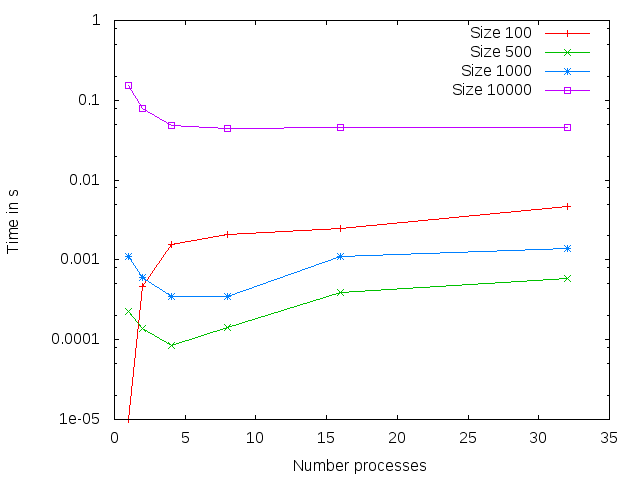
\includegraphics[width=0.7\columnwidth]{time-to-size}
\end{center}
Folgender Plot zeigt noch eine Aufstellung des Speed-Up, abhängig von der Nummer an
Prozessen. Für eine größe von 100 ist der maximale Speed-Up bei einem Thread erreicht.
Für Matrix-Größen von 500 bis 10.000 bewegt sich der Speed-Up bis 4 Threads nahe am
idealen Speed-Up. Ab 8 Threads fällt der Speed-Up jedoch selbst bei einer Matrixgrösse 
von 10.000 wieder ab.
\begin{center}
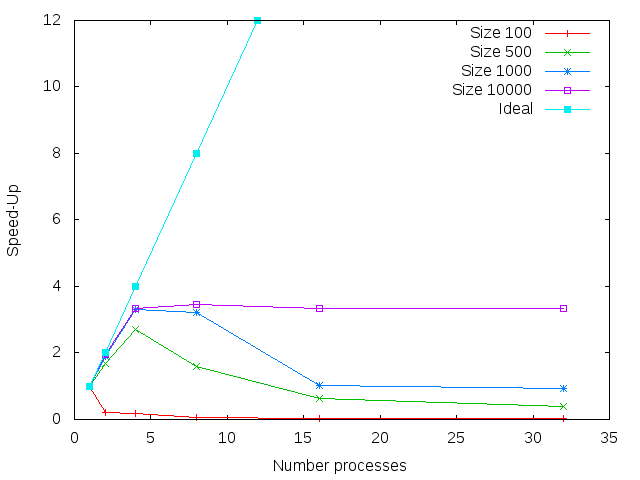
\includegraphics[width=0.7\columnwidth]{speed-up}
\end{center}
Letztendlich lässt sich sagen, dass die Ausführungsgeschwindigkeit von parallelen
Algorithmen nicht nur von der Problemgröße, sondern auch von der Anzahl der verfügbaren
Rechenresourcen abhängig ist.
\end{homeworkProblem}
\pagebreak

\end{document}
